\begin{abstract}

Si vogliono determinare gli intervalli dei valori dei tempi $T_E$ e $T_R$ per ottenere immagini MRI di un uovo pesate in $T_1$ e pesate in $T_2$. Per fare ciò si è proceduto a misurare i tempi caratteristici di albume e tuorlo separatamente tramite Inversion Recovery e CPMG. I dati sperimentali ottenuti sono stati processati e valutati tramite software UPENWin.

\end{abstract}

\section*{Introduzione}
L'esperimento effettuato si è basato sui principi della risonanza magnetica nucleare \cite{website} ed è stato realizzato secondo specifici metodi di acquisizione. 

\subsection*{Risonanza Magnetica e Rilassometria}

La risonanza magnetica nucleare è un fenomeno fisico che comporta la transizione tra stati energetici del momento angolare nucleare dei nuclei atomici.
Il fenomeno si verifica solo in presenza di nuclei atomici caratterizzati da momento angolare, che permette l'interazione con campi magnetici esterni.
La combinazione delle interazioni dei vari nuclei con lo stesso campo magnetico induce la formazione di una magnetizzazione nucleare di equilibrio, da cui è possibile ricavare informazioni sul sistema studiato.

Infatti, le informazioni si rilevano studiando il ritorno della magnetizzazione allo stato di equilibrio.
Ciò è realizzato cedendo al sistema energia in condizione di risonanza e lasciando che la magnetizzazione tenda a riportarsi allo stato d'ordine iniziale. 

All'equilibrio, la magnetizzazione nucleare è allineata con il campo magnetico uniforme applicato, detto $B_0$, e, una volta stimolato il sistema, applicando un impulso, la magnetizzazione è caratterizzata da un moto.
L'impulso esercitato equivale ad un campo magnetico stimolante, detto $B_1$, che è perpendicolare a $B_0$ ed oscillante con una frequenza pari alla frequenza di risonanza. 
L'applicazione di $B_1$ allontana la magnetizzazione dallo stato stazionario e innesca un moto per la magnetizzazione.
Il moto innescato è una combinazione di rotazioni sia attorno a $B_0$ che alla direzione di $B_1$.
La rotazione per $B_1$ permette di modificare la direzione della magnetizzazione e quindi il tempo di applicazione dell'impulso incide sulla grandezza dell'angolo di rotazione, chiamato flip angle.

Al termine dell'impulso, se il sistema si trovasse in condizioni ideali, la magnetizzazione dovrebbe continuare solo a ruotare attorno a $B_0$ alla frequenza di risonanza. 
Ciò però non si verifica a causa delle diverse posizioni degli atomi nel sistema, che comporta la percezione della non perfetta uniformità del campo magnetico $B_0$. 

In conseguenza gli atomi sono caratterizzati da diverse frequenze di rotazione dei singoli momenti angolari.
Un fenomeno di questo tipo causa una dispersione del vettore magnetizzazione sul piano perpendicolare alla direzione di $B_0$.
In questo modo il vettore magnetizzazione ritorna alla posizione di equilibrio e questo effetto è denominato rilassamento.

Il rilassamento è studiato in due componenti, la componente lungo la direzione del campo magnetico $B_0$ (a cui associamo l'asse $z$) e la componente sul piano perpendicolare (piano $xy$). 
Entrambe le componenti sono perciò caratterizzate da un relativo tempo di rilassamento, che nel caso della componente $z$ chiameremo $T_1$ e nel caso del piano $xy$ chiameremo $T_2$.
A partire dallo studio di questi due tempi di rilassamento, sono state sviluppate tecniche per l'elaborazione di immagini MRI.

Nella sezione successiva si trattano i metodi e la strumentazione adoperati in questo esperimento per la misurazione di queste due grandezze.

\subsection*{Tomografia a Risonanza Magnetica Nucleare}

Per riuscire ad ottenere un segnale NMR localizzato spazialmente si fa uso di campi magnetizi $B_0$ non uniformi lungo la coordinata $x$ e caratterizzati da un gradiente di campo magnetico lineare nella forma $B_z = B_0 + G_x x$, in questo modo si avrà come diretta conseguenza che le frequenze di Larmor dipenderanno linearmente in egual misura dalla coordinata $x$ secondo l'equazione:
\begin{equation}
	\nu(x) = \frac{\gamma}{2\pi}B_0 + \frac{\gamma}{2\pi}G_x x
\end{equation}
Sfruttando quindi gradienti lineari lungo le 3 coordinate spaziali, si possono ottenere frequenze dipendenti linearmente dalla posizione dei nuclei lungo la coordinata $x$ tramite trasformata di Fourier. Una delle sequenze di segnali più usata è la sequenza \textit{Gradient-Echo}, rappresentata in Figura \ref{fig:GEcho}.

\begin{figure}[ht]
\centering
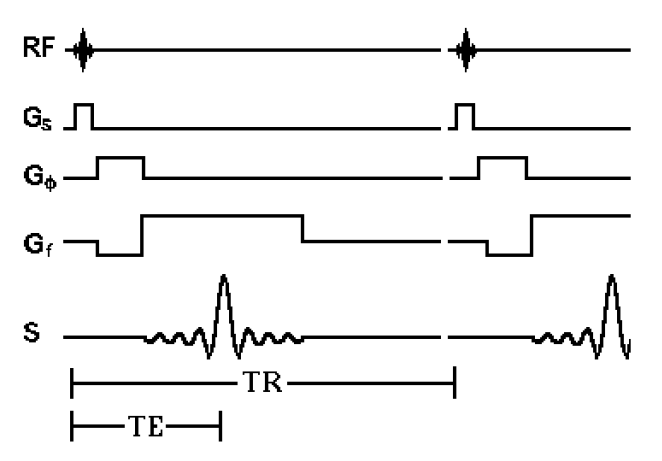
\includegraphics[width=\columnwidth]{gradient-echo.PNG}
\caption{Schema rappresentante i segnali usati in una sequenza \textit{Gradient-Echo}, un gradiente $G_s$, lungo $z$, insieme ad un impulso $RF$, seleziona la slice; un gradiente lungo $y$ codifica la fase $G_\Phi$; un gradiente lungo $x$ codifica la frequenza $G_f$. \cite{website}}
\label{fig:GEcho}
\end{figure}

Tramite il principio zeugmatografico è quindi possibile costruire una procedura di costruzione di immagini tramite risonanza magnetica. 
Tuttavia, per riuscire a tener conto delle pesature in $T_1$ ed in $T_2$ dei vari materiali, nonché evitare costanti ricollocazioni dei gradienti, si preferisce operare tramite metodo spin-warp.

\subsubsection*{Metodo spin-warp}

Con questo metodo, per definire una immagine su di un piano $(x,y)$, si comincia con l'effettuare $N_{\Phi}$ misure, ciascuna caratterizzata da un suo gradiente $G_{\Phi}$ di durata $\tau_{\Phi}$. Queste misure sono intervallate da un tempo di ripetizione $T_R$. Si acquisiscono $N_f$ dati per ogni misura (per un totale di $N_{\Phi}N_f$).

Dalla teoria \cite{dhawan2011medical} si ha che il segnale acquisito sarà proporzionale alla densità dei nuclei presenti secondo l'equazione:
\begin{multline}
	S(G_{\Phi}, \tau_{\Phi}, G_f, t) \propto\\ \int_{\text{slice}}\int_{\text{slice}} \rho(x,y) e^{-i\gamma G_\Phi y \tau_\Phi}e^{-i\gamma G_\Phi x \tau_\Phi} \, dxdy
	\label{eq:spin-warp}
\end{multline}
Trattando quindi il tutto su di uno spazio $K$, sul quale si definiscono le variabili
\begin{align}
	K_x &= \frac{\gamma}{2\pi}G_f t \\
	K_y &= \frac{\gamma}{2\pi}G_\Phi \tau_\Phi
\end{align}
si può ricavare da (\ref{eq:spin-warp}) la densità in funzione del segnale:
\begin{multline}
	\rho(x,y) \propto \\\int_{-\infty}^{+\infty}\int_{-\infty}^{+\infty} S(K_x,K_y) e^{2i\pi(K_x x +K_y y)}\, dK_x dK_y    .
\end{multline}
Variando i gradienti si riesce quindi a campionare tutto lo spazio $K$.

Per avere un buon contrasto nell'immagine, si fa uso di una sequenza a eco di spin con metodo spin-warp, la cui magnetizzazione è caratterizzata dall'equazione:
\begin{equation}
	M_{xy}{(T_R,T_E)} = M_0[1-e^{-\frac{T_R}{T_1}}(2e^{-\frac{T_{E/2}}{T_1}}-1)]e^{-\frac{T_E}{T_2}} .
\label{fm:sw}
\end{equation}
Dove i parametri fondamentali $T_E$ e $T_R$ possono essere manipolati al fine di ottenere diverse tipologie di contrasto pesato o sui tempi $T_1$ dei materiali o sui tempi $T_2$ o sulla densità protonica.% (si veda Tabella \ref{tab:peso}).

%\begin{table}
%\centering
%\begin{tabular}{l|cc}
%	\toprule
%	Densità protonica & $TE \ll T_2$	& $TR > 5T_1$ \\
%	Pesate in $T_1$   & $TE \ll T_2$	& $TR < T_1$ \\
%	Pesate in $T_2$   & $TE > T_2$		& $TR > 5T_1$ \\
%	\bottomrule
%\end{tabular}
%\caption{Impostazione dei valori $TE$ e $TR$ per diverse tipologie di pesatura.}
%\label{tab:peso}
%\end{table}